%!TEX root = alga.tex
\section{The core}\label{sec-core}

In this section we define the \emph{core} of algebraic graphs -- a minimal set
of graph construction primitives that are compositional and total. The core is
built on the \emph{algebra of parameterised graphs}, a mathematical formalism
used in hardware design~\cite{2014_algebra_mokhov},
which we distil and adapt to the context of graph representation in functional
programming languages.

Let $G$ be a set of unlabelled directed graphs whose vertices come from a fixed
universe $\mathbb{V}$. As an example, we can think of graphs whose vertices are
positive integers. A graph $g \in G$ can be represented by a pair $(V, E)$ where
$V\subseteq \mathbb{V}$ is the set of its vertices and $E \subseteq V \times V$ is
the set of its edges.
If $E \nsubseteq V \times V$, then the pair $(V, E)$ is inconsistent and does not
correspond to a graph, which often leads to partial functions, as discussed
in \S\ref{sec-motivation}.

When one needs to guarantee the internal consistency of a data structure, such
as the pair $(V, E)$, the standard solution is to define an abstract interface
that encapsulates the data structure and provides a set of safe construction
primitives. This is exactly the approach we take in this paper.

\subsection{Constructing graphs}\label{sub-constructing}

The simplest possible graph is the \emph{empty} graph. We will denote it by
$\varepsilon$, therefore $\varepsilon = (\varnothing, \varnothing)$ and
$\varepsilon \in G$. A graph with a \emph{single vertex} $v \in \mathbb{V}$
will be denoted simply by $v$. For example, $1 \in G$ is the graph
$({1}, \varnothing)$.

To construct larger graphs from the above primitives we define binary
operations \emph{overlay} and \emph{connect}, denoted by $+$ and $\rightarrow$,
respectively. The overlay operation $+$ is defined as
\[
(V_1, E_1) + (V_2, E_2)~~\defeq~~(V_1 \cup V_2, E_1 \cup E_2).
\]
That is, the overlay of two graphs comprises the union of their vertices and edges.

The connect $\rightarrow$ operation is defined in a similar manner:
\[
(V_1, E_1) \rightarrow (V_2, E_2)~~\defeq~~(V_1 \cup V_2, E_1 \cup E_2 \cup V_1 \times V_2).
\]
The difference is that when we connect two graphs, an edge is added from each
vertex of the left-hand argument to each vertex of the right-hand
argument\footnote{Our definitions of overlay and connect coincide
with those of graph \emph{union} and \emph{join}, respectively,
e.g see Harary~\citeyear{1969_graph_theory_harary},
however the arguments of union and join are typically assumed to have disjoint
sets of vertices. We make no such assumptions, hence our definitions are total:
any two graphs can be composed using overlay and connect.
}.
Note that the connect operation is the only source of edges when constructing
graphs. As we will see in \S\ref{sec-algebra}, the overlay and connect are very
similar to addition and multiplication, therefore connect has a higher
precedence, i.e. $1 + 2 \rightarrow 3$ is interpreted as $1 + (2 \rightarrow 3)$.

\noindent
Fig.~\ref{fig-construction} illustrates a few examples of constructing graphs
using the defined primitives:
\begin{itemize}
  \item $1 + 2$ is the graph with two isolated vertices 1 and 2.
  \item $1 \rightarrow 2$ is the graph with an edge between vertices 1
  and 2, i.e. the graph $a$ from Fig.~\ref{fig-example}.
  \item $1 \rightarrow (2 + 3)$ is the graph with three vertices $\{1, 2, 3\}$
  and two edges $(1, 2)$ and $(1, 3)$.
  \item $1 \rightarrow 1$ is the graph with vertex 1 and the \emph{self-loop}
  going from the vertex to itself.
  \item $1 \rightarrow 2 + 3 \rightarrow 1$ is the graph $b$ from
  Fig.~\ref{fig-example}.
\end{itemize}

\begin{figure}
\hspace{-5mm}
\begin{subfigure}[b]{0.2\linewidth}
\centerline{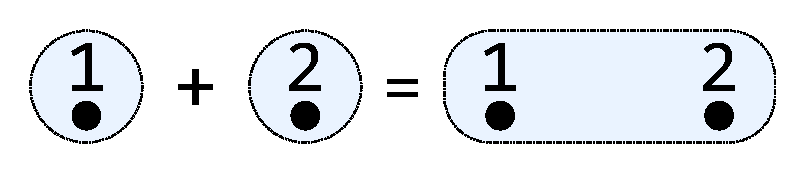
\includegraphics[scale=0.27]{fig/ex-a.pdf}}
\vspace{-2.4mm}
\caption{$1 + 2$}
\centerline{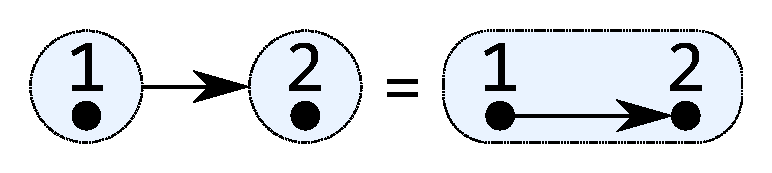
\includegraphics[scale=0.27]{fig/ex-b.pdf}}
\vspace{-2.4mm}
\caption{$1 \rightarrow 2$}
\end{subfigure}
\hspace{11mm}
\begin{subfigure}[b]{0.17\linewidth}
\centerline{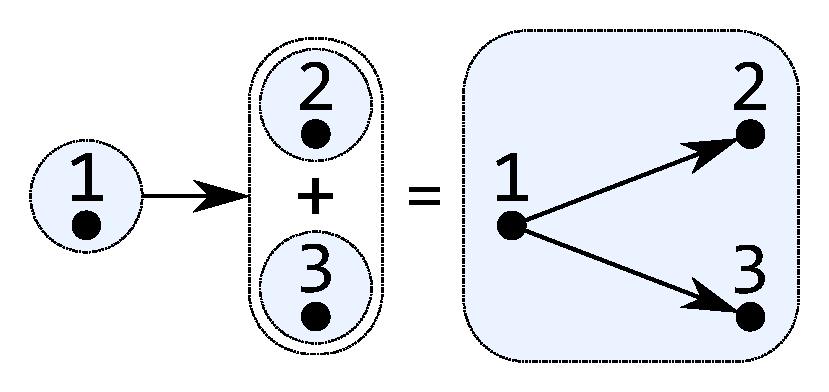
\includegraphics[scale=0.27]{fig/ex-c.pdf}}
\vspace{-1mm}
\caption{$1 \rightarrow (2 + 3)$}
\end{subfigure}
\hspace{12mm}
\begin{subfigure}[b]{0.15\linewidth}
\centerline{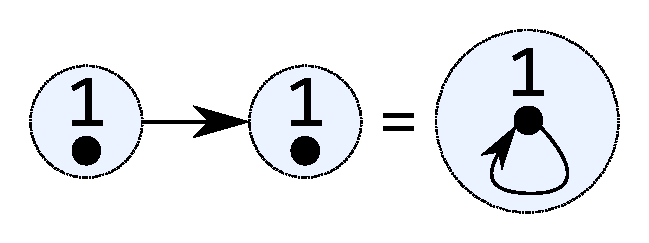
\includegraphics[scale=0.27]{fig/ex-d.pdf}}
\vspace{2.4mm}
\caption{$1 \rightarrow 1$}
\end{subfigure}
\hspace{12mm}
\begin{subfigure}[b]{0.2\linewidth}
\centerline{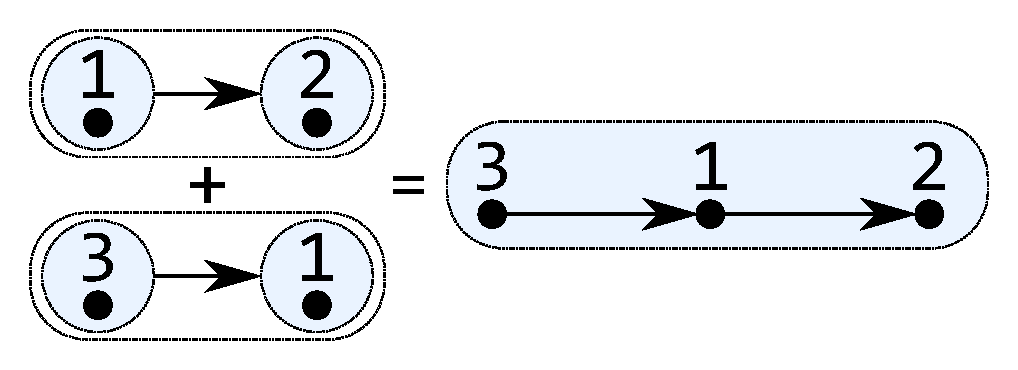
\includegraphics[scale=0.27]{fig/ex-e.pdf}}
\vspace{-1mm}
\caption{$1 \rightarrow 2 + 3 \rightarrow 1$}
\end{subfigure}
\vspace{-1mm}
\caption{Examples of graph construction\label{fig-construction}}
\vspace{-3mm}
\end{figure}

\vspace{-1mm}
\subsection{Type class}\label{sub-class}

We abstract the graph construction primitives defined in \S\ref{sub-constructing}
as the type class \hs{Graph}:

\begin{minted}{haskell}
class Graph g where
    type Vertex g
    empty   :: g
    vertex  :: Vertex g -> g
    overlay :: g -> g -> g
    connect :: g -> g -> g
\end{minted}

\noindent
Here the associated type\footnote{Associated
types~\cite{2005_associated_type_chakravarty} require the \textsf{TypeFamilies}
GHC extension.} \hs{Vertex@\,@g} corresponds to the universe of graph
vertices $\mathbb{V}$, \hs{empty} is the empty graph
$\varepsilon$, \hs{vertex} constructs a graph with a single vertex,
and \hs{overlay} and \hs{connect} compose given graphs according to
the definitions in~\S\ref{sub-constructing}. All methods of the type class
are total, i.e. are defined for all possible inputs, therefore,
the presented API allows \emph{fewer opportunities for usage errors}
and \emph{greater opportunities for reuse}.

Let's put the API to the test and construct some graphs! A single edge is
obtained by connecting two vertices:

\begin{minted}{haskell}
edge :: Graph g => Vertex g -> Vertex g -> g
edge x y = connect (vertex x) (vertex y)
\end{minted}

\noindent
The graphs in Fig.~\ref{fig-construction}(b,d) are \hs{edge@\,@1@\,@2} and
\hs{edge@\,@1@\,@1}, respectively.
A graph that contains a given list of isolated vertices can be constructed
as follows:

\begin{minted}{haskell}
vertices :: Graph g => [Vertex g] -> g
vertices = @\std{foldr}@ overlay empty . @\std{map}@ vertex
\end{minted}

\noindent
That is, we turn each vertex into a singleton graph and overlay the results.
The graph in Fig.~\ref{fig-construction}(a) is \hs{vertices@\,@[1,2]}.
By replacing \hs{overlay} with \hs{connect} in the above
function, we obtain a \emph{clique} -- a fully connected graph on a given list
of vertices:

\begin{minted}{haskell}
clique :: Graph g => [Vertex g] -> g
clique = @\std{foldr}@ connect empty . @\std{map}@ vertex
\end{minted}

\noindent
For example, the infinite clique on all positive integers is \hs{clique@\,@[1..]}.

The above graph construction functions are total, fully polymorphic, and elegant.
Thanks to the minimalistic core type class, it is easy to wrap your favourite
graph library into the described interface, and reuse these functions, as well
as many others that we define throughout this paper.
